\documentclass[12pt, letterpaper]{article}
\usepackage{amsmath}
\usepackage{amssymb}
\usepackage[finnish,english]{babel}
\usepackage{braket}
\usepackage{fancyhdr}
\usepackage{geometry}
\usepackage{graphicx}
\usepackage{listings}
\usepackage{mathtools}
\usepackage{paracol}
\usepackage{physics}
\usepackage{titlesec}
\usepackage{tikz-feynman}
\usepackage{import}
\usepackage{xifthen}
\usepackage{pdfpages}
\usepackage{transparent}
\usepackage[many]{tcolorbox}

\newcommand{\N}{\mathbb{N}}
\newcommand{\Z}{\mathbb{Z}}
\newcommand{\Q}{\mathbb{Q}}
\newcommand{\R}{\mathbb{R}}
\newcommand{\C}{\mathbb{C}}

\newcommand{\incfig}[2][1]{%
  \def\svgwidth{#1\columnwidth}
  \import{./figures/}{#2.pdf_tex}
}

\pdfsuppresswarningpagegroup=1

%\geometry{a4paper, total={170mm,257mm}, left=20mm, top=20mm,}
\newcommand{\dbar}{\dd\hspace*{-0.18em}\bar{}\hspace*{0.1em}}

\definecolor{backcolour}{rgb}{0.25,0.25,0.22}
\definecolor{codegreen}{rgb}{0.5,0.9,0.6}
\definecolor{codegray}{rgb}{0.5,0.5,0.5}
\definecolor{codepurple}{rgb}{0.58,0,0.82}
\definecolor{codebeige}{rgb}{0.90,0.80,0.55}

\tcolorboxenvironment{lstlisting}{
  spartan,
  frame empty,
  boxsep=0mm,
  left=1mm,right=1mm,top=-1mm,bottom=-1mm,
  colback=backcolour,
}

\lstdefinestyle{mystyle}{
    backgroundcolor=\color{backcolour},
    commentstyle=\color{gray},
    keywordstyle=\color{codebeige},
    numberstyle=\tiny\color{codegray},
    stringstyle=\color{codegreen},
    basicstyle=\ttfamily\footnotesize\color{white},
    breakatwhitespace=false,
    breaklines=true,
    captionpos=b,
    keepspaces=true,
    numbers=none,
    numbersep=5pt,
    showspaces=false,
    showstringspaces=false,
    showtabs=false,
    tabsize=2
}

\lstset{style=mystyle}


\author{Tom Rindell}
\title{}

\pagestyle{fancy}
\pagenumbering{gobble}

\rhead{\textsc{NMSC\\Final Project}}
%\rhead{\textsc{Tools of HPC\\Exercise 2}}
\lhead{\textsc{Tom Rindell\\014605789}}


\begin{document}
Instructions for writing the report: Explain what your learned in step 1 in the methods section. In the results
section, include the visualizations from Task 4, and your own setup from Task 5, and return the commented code
with compilation and usage instructions. If you encounter issues implementing the code in Tasks 2–5, you can
instead focus on clearly explaining the algorithm and describing the difficulties you faced. Alternatively, if you
successfully implemented the code but struggled to understand the algorithm, emphasize presenting and analyzing
your results. The emphasis on an ideal report is explaining the algorithm well (while containing all the asked
results), but a limited report is better than no report.

\section{Introduction}
This project studies an implementation of fluid flow simulation developed by Jos Stam %\citep{}.
(trading off accuracy for stability and efficiency)

\section{Methods}
\begin{align*}
  \nabla\cdot\vb{u} &= 0 \\
  \frac{\partial\vb{u}}{\partial t} &= -(\vb{u}\cdot \nabla)\vb{u}-\frac{1}{\rho}\nabla p + \nu \nabla^{2}\vb{u} + \vb{f}
  \\\frac{\partial\vb{u}}{\partial t} &= \left( (\nu \nabla-\vb{u} )\cdot \nabla\right) \vb{u}-  \nabla \left(\frac{p}{\rho} + U\right)
  \\\frac{\partial{u_{x}}}{\partial t} &= -{u}_{x} \nabla{u_{x}}+  \frac{\partial}{\partial x} \left(\nu\nabla{u_{x}}-  \frac{p}{\rho} - U\right)
\end{align*}

\section{Implementation}
Two sets of $N\times N$ grids are allocated.

The first stores the initial values at the beginning of an iteration whereas the updated values are stored in the second set of grids.
On the next iteration the roles are swapped; what was the second set of grids now functions as the set of initial values and the updated values are stored into the first set of grids.

Fluid flow solver used here is a slightly altered version of the code from Stam's paper %\citep{}.


\section{Results}
\begin{figure}[h!]
  \center
  
\includegraphics[width=8em]{run/images/10_steps.png}
  
\includegraphics[width=8em]{run/images/100_steps.png}
  
\includegraphics[width=8em]{run/images/300_steps.png}
  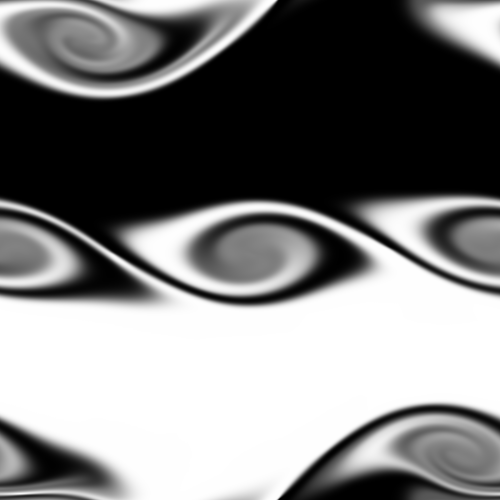
\includegraphics[width=8em]{run/images/500_steps.png}
  \caption{}
\end{figure}

\section{Conclusions}

\section{References}

\end{document}

